\documentclass[aspectratio=169]{beamer}
\usetheme{Madrid}
\usecolortheme{default}
\usepackage{amsmath, amssymb, bm}
\usepackage{graphicx}
\usepackage{booktabs}
\usepackage{tikz}
\usepackage{array}
\usepackage{multicol}
\usepackage{ragged2e}

\definecolor{accent}{RGB}{38,70,83}
\definecolor{accent2}{RGB}{42,157,143}
\definecolor{accent3}{RGB}{233,196,106}
\definecolor{accent4}{RGB}{231,111,81}

\setbeamercolor{structure}{fg=accent}
\setbeamercolor{title}{fg=white,bg=accent}
\setbeamercolor{frametitle}{fg=white,bg=accent}
\setbeamercolor{block title}{fg=white,bg=accent2}
\setbeamercolor{block body}{fg=black,bg=accent2!8}
\setbeamercolor{alerted text}{fg=accent4}
\setbeamertemplate{navigation symbols}{}
\setbeamertemplate{footline}{}

\title{Spot Detection from Averaged TIFF Frames}
\subtitle{Richardson--Lucy Deconvolution + Gaussian Component Fitting}
\author{}
\date{}

\begin{document}

\begin{frame}
    \titlepage
    \vspace{-0.4em}
    \begin{center}
        \small Pipeline summary prepared for Overleaf from the uploaded Python workflow and result figures.
    \end{center}
\end{frame}

\begin{frame}{Objective and workflow}
\begin{columns}[T,totalwidth=\textwidth]
\column{0.58\textwidth}
\begin{block}{Goal}
Detect point-like emitters in a noisy image stack, then decide whether each bright region contains \textbf{one} spot or \textbf{two overlapping} spots.
\end{block}

\begin{block}{Processing pipeline}
\small
\begin{enumerate}
    \item Load \textbf{50 cropped TIFF frames} and compute the average image.
    \item Build a \textbf{Gaussian PSF} and apply Richardson--Lucy deconvolution.
    \item Threshold the deconvolved image, label connected components, and crop local ROIs.
    \item Fit \textbf{1-Gaussian} and \textbf{2-Gaussian} models; use BIC to keep the simpler or split model.
\end{enumerate}
\end{block}

\column{0.38\textwidth}
\begin{block}{Key settings}
\small
\begin{tabular}{>{\bfseries}p{0.48\linewidth}p{0.38\linewidth}}
Frames & 50 \\
RL iterations & 10 \\
PSF size & 15 $\times$ 15 \\
PSF $\sigma$ & 2.0 px \\
Threshold & 0.02 \\
ROI pad & 4 px \\
BIC margin & 25 \\
Min separation & 5 px \\
\end{tabular}
\end{block}

\vspace{0.3em}
\begin{alertblock}{Main outcome}
\centering
\Large \textbf{19 final spot centroids}
\end{alertblock}
\end{columns}
\end{frame}

\begin{frame}{Preprocessing and deconvolution}
\begin{columns}[T,totalwidth=\textwidth]
\column{0.56\textwidth}
\begin{block}{Stack averaging}
\[
\bar{I}(x,y)=\frac{1}{N}\sum_{k=1}^{N} I_k(x,y), \qquad N=50
\]
Averaging reduces frame-to-frame noise before spot enhancement.
\end{block}

\begin{block}{Gaussian PSF + RL sharpening}
\[
\mathrm{PSF}(x,y) \propto \exp\!\left(-\frac{x^2+y^2}{2\sigma^2}\right), \qquad \sigma=2.0
\]
The averaged image is normalized to $[0,1]$ and processed with \textbf{10 Richardson--Lucy iterations}.
\end{block}

\begin{itemize}
    \item RL helps sharpen blurred emitters.
    \item Better localization improves later thresholding and fitting.
    \item The deconvolved image is the input for segmentation.
\end{itemize}

\column{0.40\textwidth}
\begin{block}{Why this matters}
\small
Direct thresholding on raw averaged data can merge nearby emitters.\medskip

Deconvolution increases local contrast, making it easier to isolate candidate spots before model fitting.
\end{block}

\vspace{0.5em}
\begin{block}{Implementation note}
\small RL is applied with a Gaussian PSF generated directly in the script.
\end{block}
\end{columns}
\end{frame}

\begin{frame}{Thresholding and connected-component detection}
\begin{columns}[T,totalwidth=\textwidth]
\column{0.44\textwidth}
\begin{block}{Binary mask}
\[
M(x,y)=\mathbf{1}\!\left[\mathrm{RL}(x,y) > 0.02\right]
\]
Only pixels above threshold are retained as candidate signal.
\end{block}

\begin{block}{Component filtering}
\begin{itemize}
    \item Connected components are labeled with \texttt{ndi.label}.
    \item Valid area range: \textbf{3 to 10{,}000 pixels}.
    \item Each accepted region is expanded by \textbf{4 pixels} on each side.
\end{itemize}
\end{block}

\column{0.52\textwidth}
\centering
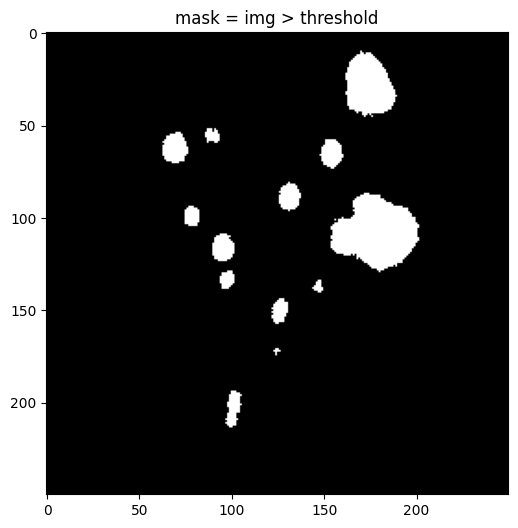
\includegraphics[width=\linewidth]{threshold_mask.png}

\vspace{0.4em}
\scriptsize Thresholded mask after RL deconvolution. White regions are the connected components passed to local fitting.
\end{columns}
\end{frame}

\begin{frame}{Local Gaussian fitting and model selection}
\begin{columns}[T,totalwidth=\textwidth]
\column{0.56\textwidth}
\begin{block}{Competing models per ROI}
\small
Single spot:
\[
G_1 = A_1 e^{-\frac{(x-x_{01})^2+(y-y_{01})^2}{2s_1^2}} + B
\]
Two spots:
\[
G_2 = G_A + G_B + B
\]
Each Gaussian has its own amplitude, center, and width.
\end{block}

\begin{block}{Interpretation}
\small
A bright blob is split into two emitters only when the data support a meaningful improvement.
\end{block}

\column{0.40\textwidth}
\begin{block}{BIC-based decision rule}
\small
\[
\mathrm{BIC} = n\ln\!\left(\frac{\mathrm{RSS}}{n}\right)+k\ln(n)
\]
Choose the two-spot model only if
\[
\mathrm{BIC}_2 < \mathrm{BIC}_1 - 25
\]
and the fitted separation is at least \textbf{5 pixels}.
\end{block}

\begin{block}{Why this helps}
\small
\begin{itemize}
    \item Penalizes unnecessary extra parameters
    \item Reduces over-splitting while keeping overlaps resolvable
\end{itemize}
\end{block}
\end{columns}
\end{frame}

\begin{frame}{Detection results and next steps}
\begin{columns}[T,totalwidth=\textwidth]
\column{0.58\textwidth}
\centering
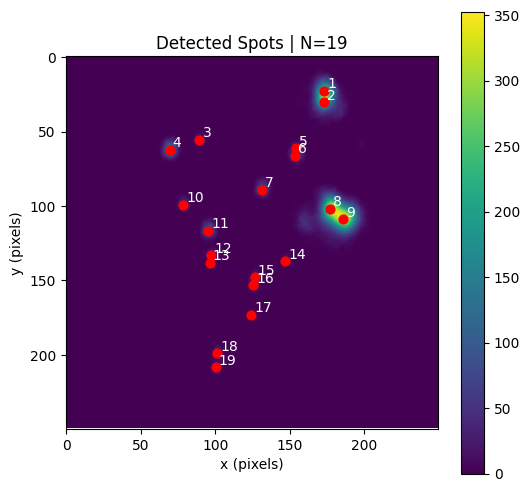
\includegraphics[width=0.95\linewidth]{detected_spots.png}

\column{0.38\textwidth}
\scriptsize
\begin{block}{Key observations}
\begin{itemize}
    \item Final count: \textbf{19 centroids}
    \item Larger bright regions can split into multiple emitters when the 2-Gaussian model is justified.
    \item The code checks close-pair distances for \textbf{(15,16)} and \textbf{(18,19)}.
\end{itemize}
\end{block}

\begin{block}{Next steps}
\begin{itemize}
    \item Validate against manual labels or simulated ground truth.
    \item Test sensitivity to threshold, PSF width, and RL iterations.
    \item Export centroid tables for downstream analysis.
\end{itemize}
\end{block}
\end{columns}
\end{frame}

\end{document}
